\documentclass[a4paper]{article}
\usepackage{amsfonts}
\usepackage{amsmath}
\usepackage{amssymb}
\usepackage{graphicx}
\usepackage{extarrows}

\newcommand{\integral}{\displaystyle\int}
\newcommand{\limit}{\lim\limits}

\begin{document}

\noindent \large Auteur: Seda Jusjajeva\\
\noindent \large Studierichting: Informatica\\
\noindent \large Oefeningenreeks 5D nr. 1.2\\

\medskip

\normalsize



$\integral_{-2}^1 (x^3 - x)dx$ \\

$\integral (x^3 - x)dx = \integral x^3dx - \integral xdx = \dfrac{x^4}{4} - \dfrac{x^2}{2} + c = \dfrac{x^4 - 2x^2}{4} + c$ \\

Grafiek: \\

\begin{figure}[h]
\centering
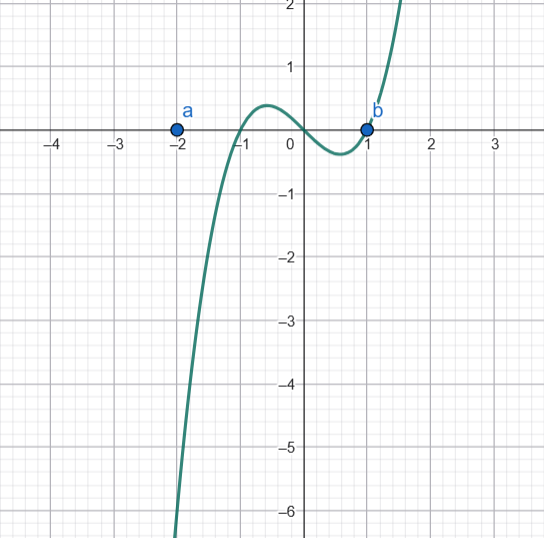
\includegraphics[width=6cm]{5D-1.2-seda.jusjajeva.INF.png}
\end{figure}

$\Rightarrow \integral_{-2}^1 (x^3 - x)dx = -\integral_{-2}^{-1} (x^3 - x)dx + \integral_{-1}^0 (x^3 - x)dx - \integral_{0}^1 (x^3 - x)dx$ \\

$= -\left[\dfrac{x^4 - 2x^2}{4}\right]_{-2}^{-1} + \left[\dfrac{x^4 - 2x^2}{4}\right]_{-1}^{0} - \left[\dfrac{x^4 - 2x^2}{4}\right]_{0}^{1}$ \\

$= -\left(\dfrac{1 - 2}{4} - \dfrac{2^4 - 2(2)^2}{4}\right) + \left(0 - \dfrac{1 - 2}{4}\right) - \left(\dfrac{1 - 2}{4} - 0\right)$ \\

$= \dfrac{9}{4} - \dfrac{1}{4} + \dfrac{1}{4}$ \\

$= \dfrac{11}{4}$ \\




\begin{thebibliography}{999}
%\bibitem{a} Referentie
\end{thebibliography}
\end{document}